\documentclass[t]{beamer}

\usepackage[utf8x]{inputenc}
\usepackage{xskak,chessboard} % for chess positions
\usepackage{wasysym} % for custom chess pieces in masks
\usepackage{graphicx}

\setbeamercovered{transparent}
\setbeamersize{text margin left=1em, text margin right=0em}
\setbeamertemplate{sidebar right}{}
\setbeamertemplate{footline}{\hfill\insertframenumber{}~~~}
\setbeamercovered{invisible}

\setbeamertemplate{subsection in toc}[square]
\AtBeginSubsection[]
{
 \begin{frame}<beamer>
 \frametitle{Overview}
 \tableofcontents[currentsubsection]
 \end{frame}
}

\usepackage{listings}

\usepackage{listings}
\lstdefinelanguage{ReactiveML}
  {morekeywords={assert,asr,class,closed,constraint,external,%
      functor,include,inherit,land,lazy,lor,lsl,lsr,lxor,method,mod,%
      module,new,open,parser,private,sig,struct,val,virtual,when,%
      object,%
      and,as,begin,do,done,dopar,downto,else,end,exception,for,%
      fun,function,if,in,let,match,mutable,of,rec,then,%
      to,try,type,while,with,%
      process,emit,await,signal,default,gather,present,control,until,%
      loop,nothing,pause,pre,run,immediate,one.last},%
   sensitive,%
   morecomment=[n]{(*}{*)},%
   morestring=[b]",%
   moredelim=*[directive]\#,%
   moredirectives={open,close,include}%
  }[keywords,comments,strings,directives]%

% \lstset{language=ReactiveML,%
%    basicstyle=\ttfamily,%
%    keywordstyle=\bfseries\rmfamily,%
%    columns=fullflexible,%
%    moredelim=[is][\itshape]{\#}{\#}%
% }

\lstset{language=ReactiveML,%
   basicstyle=\ttfamily,%
   keywordstyle=\ttfamily,%
   columns=fullflexible,%
   moredelim=[is][\itshape]{\#}{\#}%
}

% \usepackage{alltt}
% \newenvironment{lstlisting}%
% {\begin{alltt}}%
% {\end{alltt}}

%%% Local Variables: 
%%% mode: latex
%%% TeX-master: "these"
%%% End: 

\lstset{language=ReactiveML,%
   basicstyle=\ttfamily,%
   keywordstyle=\color{blue}\ttfamily,%
   columns=fullflexible,%
   moredelim=[is][\itshape]{\#}{\#},%
   showstringspaces=false,%
}
\lstnewenvironment{lstrml}%
{\footnotesize \lstset{language=ReactiveML,keepspaces=true}}
{}
\lstnewenvironment{lstpython}%
{\footnotesize \lstset{language=Python,keepspaces=true}}
{}

\title{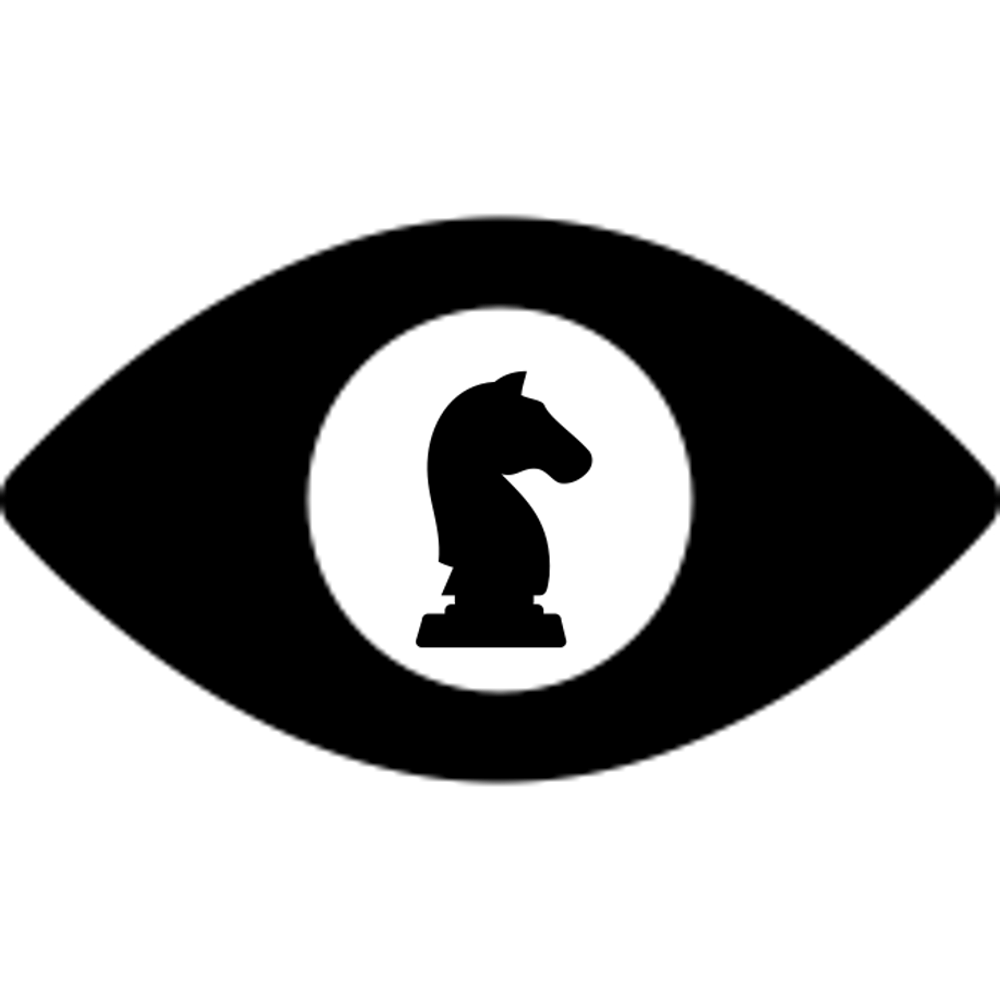
\includegraphics[scale=0.1]{figures/chesseye}
  \\
  ChessEye}
\author{Louis Mandel \and J{\'e}r{\^o}me Sim{\'e}on \and Philippe Suter}
\date{Palaver \\ July 12, 2016}

%% Chess diagrams

\begin{document}

%%%%%%%%%%%%%%%%%%%%%%%%%%%%%%%%%%%%%%%%%%%%%%%%%%%%%%%%%%%%%%%%%%%%%%%%%%%

\begin{frame}
  \titlepage
\end{frame}

%%%%%%%%%%%%%%%%%%%%%%%%%%%%%%%%%%%%%%%%%%%%%%%%%%%%%%%%%%%%%%%%%%%%%%%%%%%

% \begin{frame}
%   \tableofcontents
% \end{frame}

%%%%%%%%%%%%%%%%%%%%%%%%%%%%%%%%%%%%%%%%%%%%%%%%%%%%%%%%%%%%%%%%%%%%%%%%%%%

\begin{frame}[fragile]
\frametitle{Architecture}

\begin{center}
  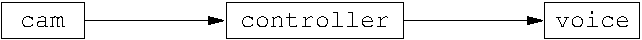
\includegraphics[scale=0.9]{figures/architecture}
\end{center}
\medskip

{\small
\begin{verbatim}
$ python cam/chesseye.py --src=1 \
    | controller/controller -kibbitz 1 \
    | python voice/speak.py
\end{verbatim}
}

\end{frame}


%%%%%%%%%%%%%%%%%%%%%%%%%%%%%%%%%%%%%%%%%%%%%%%%%%%%%%%%%%%%%%%%%%%%%%%%%%%
\section{Vision}
%%%%%%%%%%%%%%%%%%%%%%%%%%%%%%%%%%%%%%%%%%%%%%%%%%%%%%%%%%%%%%%%%%%%%%%%%%%

\begin{frame}[fragile]
\frametitle{Vision}

\vfill

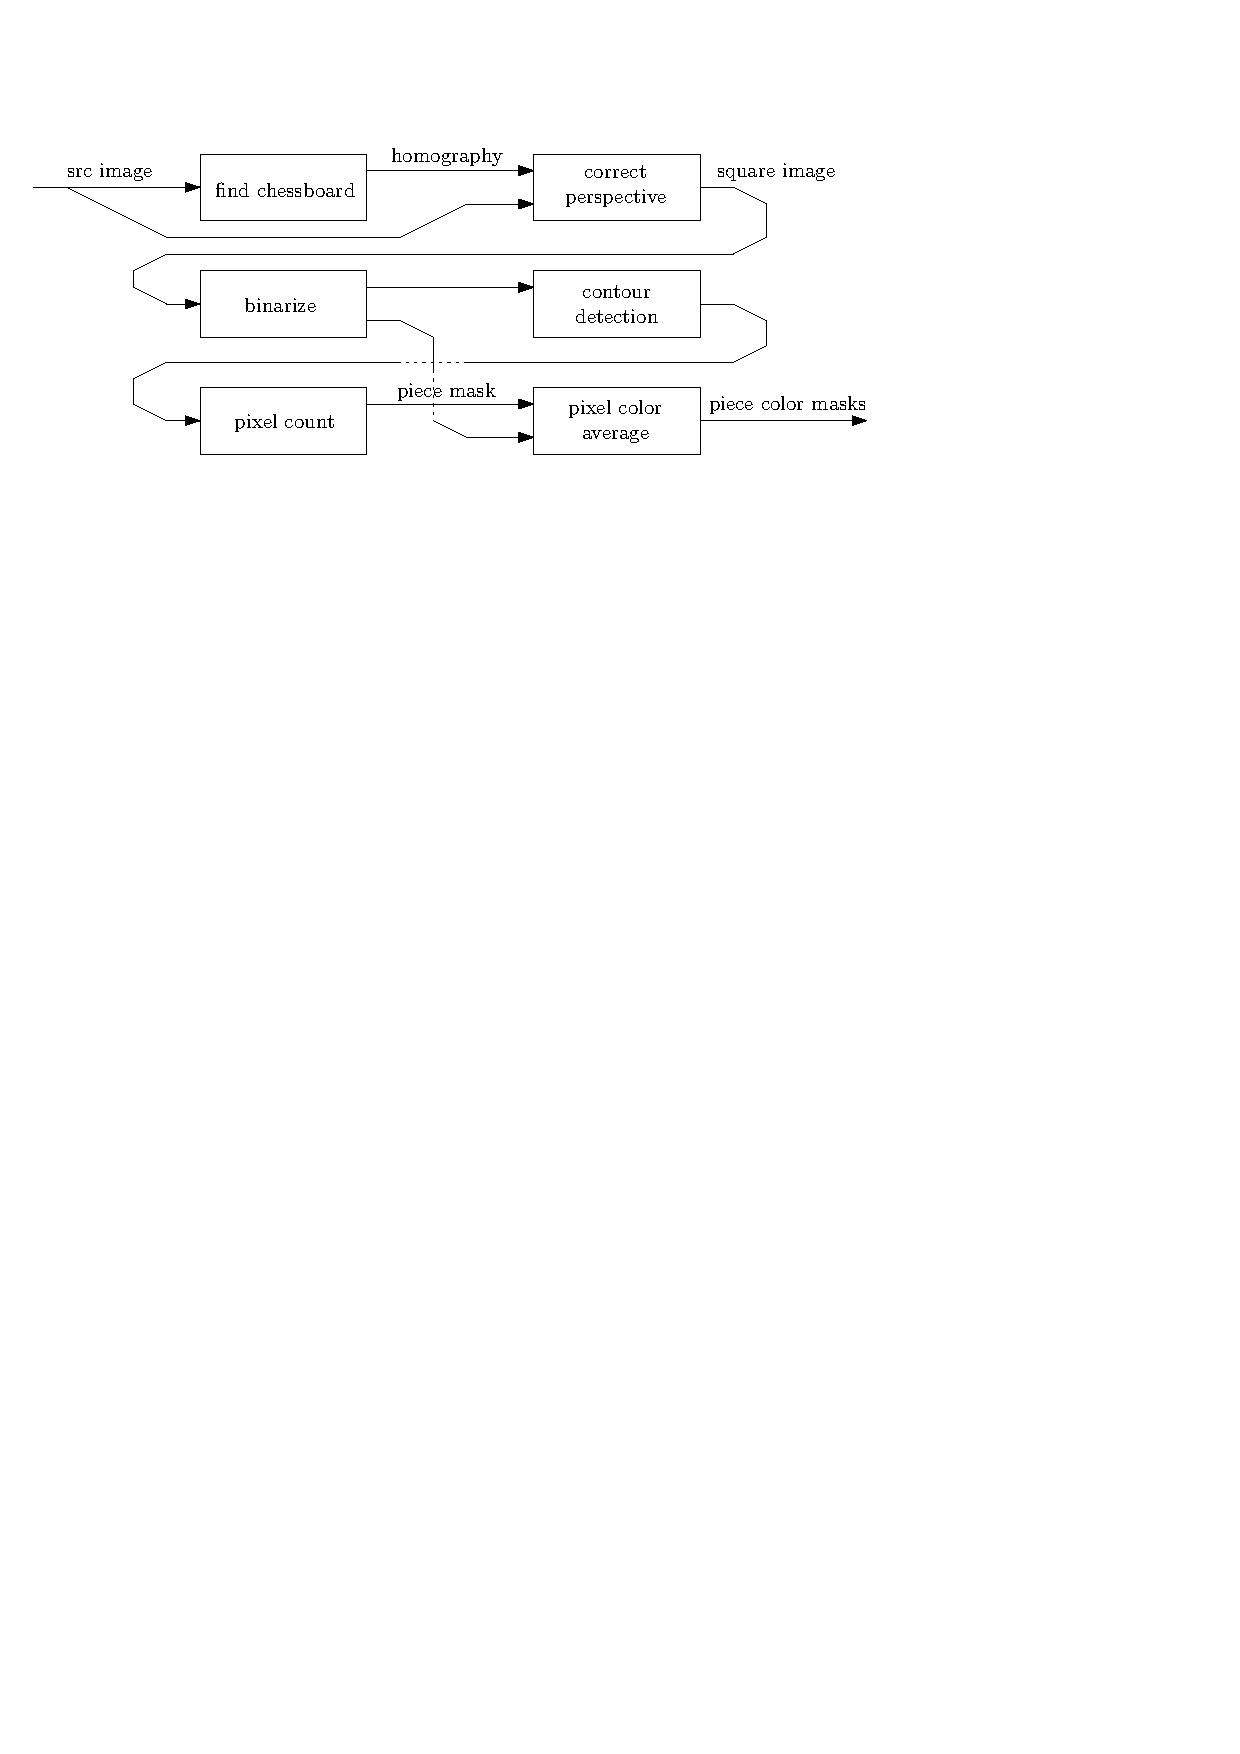
\includegraphics[scale=0.8]{figures/diagram}

\vfill

\end{frame}


%%%%%%%%%%%%%%%%%%%%%%%%%%%%%%%%%%%%%%%%%%%%%%%%%%%%%%%%%%%%%%%%%%%%%%%%%%%
\section{MaskToPosition}
%%%%%%%%%%%%%%%%%%%%%%%%%%%%%%%%%%%%%%%%%%%%%%%%%%%%%%%%%%%%%%%%%%%%%%%%%%%

%% Setup chessboard
\makeatletter
\cbDefineNewPiece{white}{C}
                 {\raisebox{0.08cm}{\cfss@whitepiececolor
                     $\Circle$}}
                 {\BlackEmptySquare%
                   \makebox[0pt][r]{\cfss@whitepiececolor
                     \raisebox{0.08cm}{%
                       \makebox[1em]{$\Circle$}}}}
\cbDefineNewPiece{black}{c}
                 {\raisebox{0.08cm}{\cfss@blackpiececolor
                     $\CIRCLE$}}
                 {\BlackEmptySquare%
                   \makebox[0pt][r]{\cfss@blackpiececolor
                     \raisebox{0.08cm}{%
                       \makebox[1em]{$\CIRCLE$}}}}
\makeatother
\setchessboard{tinyboard}

\begin{frame}[fragile]
\frametitle{Mask to position: Initial}

%%
\begin{tabular}{ccc}
\newchessgame
\chessboard[addpieces={Ca1,Cb1,Cc1,Cd1,Ce1,Cf1,Cg1,Ch1,Ca2,Cb2,Cc2,Cd2,Ce2,Cf2,Cg2,Ch2,
    ca8,cb8,cc8,cd8,ce8,cf8,cg8,ch8,ca7,cb7,cc7,cd7,ce7,cf7,cg7,ch7}]
&\raisebox{1.3cm}{$\Longrightarrow$}&
\chessboard
\end{tabular}

\hidemoves{1. e4}
\begin{tabular}{ccc}
\chessboard[addpieces={Ca1,Cb1,Cc1,Cd1,Ce1,Cf1,Cg1,Ch1,Ca2,Cb2,Cc2,Cd2,Ce4,Cf2,Cg2,Ch2,
    ca8,cb8,cc8,cd8,ce8,cf8,cg8,ch8,ca7,cb7,cc7,cd7,ce7,cf7,cg7,ch7}]
&\raisebox{1.3cm}{$\Longrightarrow$}&
\raisebox{1.3cm}{\hspace*{1.3cm}{\Large ?}}
\end{tabular}

\end{frame}

\begin{frame}[fragile]
\frametitle{Mask to position: Move}

%%
\begin{tabular}{ccc}
\chessboard[hideranks={1,2,7,8},pgfstyle=border,color=red,markfields={e2,e4},addpieces={Ce4}]
&\raisebox{1.3cm}{$\Longrightarrow$}&
\chessboard[hideranks={1,2,7,8},pgfstyle=straightmove,markmoves={e2-e4}]
\end{tabular}

\begin{tabular}{ccc}
\newchessgame
\chessboard
\hidemoves{1. e4}
&\raisebox{1.3cm}{$\Longrightarrow$}&
\chessboard[pgfstyle=straightmove,markmoves={e2-e4}]
\end{tabular}

\end{frame}

\begin{frame}[fragile]
\frametitle{Mask to position: Capture}

%%
\newgame\longmoves
{\small \mainline{1.ce4 ce5 2.Nf3 Nf6 3. d4 d6}}
\begin{tabular}{ccc}
\chessboard[addpieces={Ca1,Cb1,Cc1,Cd1,Ce1,Cf1,Cf3,Ch1,Ca2,Cb2,Cc2,Cd4,Ce4,Cf2,Cg2,Ch2,
    ca8,cb8,cc8,cd8,ce8,cf8,cf6,ch8,ca7,cb7,cc7,cd6,ce5,cf7,cg7,ch7}]
&\raisebox{1.3cm}{$\Longrightarrow$}&
\chessboard
\end{tabular}

%%
\hidemoves{4. dxe5}
\begin{tabular}{ccc}
\chessboard[pgfstyle=border,color=red,markfields={d4,e5},addpieces={Ca1,Cb1,Cc1,Cd1,Ce1,Cf1,Cf3,Ch1,Ca2,Cb2,Cc2,Ce5,Ce4,Cf2,Cg2,Ch2,
    ca8,cb8,cc8,cd8,ce8,cf8,cf6,ch8,ca7,cb7,cc7,cd6,cf7,cg7,ch7}]
&\raisebox{1.3cm}{$\Longrightarrow$}&
\chessboard[pgfstyle=straightmove,markmoves={d4-e5}]
\end{tabular}

\end{frame}

\begin{frame}[fragile]
\frametitle{Mask to position: Capture \emph{en passant}}

%%
\newgame\longmoves
{\small \mainline{1.ce4 ce5 2.Nf3 Nf6 3. d4 d6 4. d5 c5}}
    
\begin{tabular}{ccc}
\chessboard[addpieces={Ca1,Cb1,Cc1,Cd1,Ce1,Cf1,Cf3,Ch1,Ca2,Cb2,Cc2,Cd5,Ce4,Cf2,Cg2,Ch2,
    ca8,cb8,cc8,cd8,ce8,cf8,cf6,ch8,ca7,cb7,cc5,cd6,ce5,cf7,cg7,ch7}]
&\raisebox{1.3cm}{$\Longrightarrow$}&
\chessboard
\end{tabular}

%%
\hidemoves{5. dxc6...}
\begin{tabular}{ccc}
\chessboard[pgfstyle=border,color=red,markfields={d5,c5,c6},addpieces={Ca1,Cb1,Cc1,Cd1,Ce1,Cf1,Cf3,Ch1,Ca2,Cb2,Cc2,Cc6,Ce4,Cf2,Cg2,Ch2,
    ca8,cb8,cc8,cd8,ce8,cf8,cf6,ch8,ca7,cb7,cd6,ce5,cf7,cg7,ch7}]
&\raisebox{1.3cm}{$\Longrightarrow$}&
\chessboard[pgfstyle=straightmove,markmoves={d5-c6}]
\end{tabular}

\end{frame}

\begin{frame}[fragile]
\frametitle{Mask to position: Castling \& Promotion}

%%
{\small \mainline{5... Be7}}
\newgame\longmoves
{\small \hidemoves{1.ce4 ce5 2.Nf3 Nf6 3. d4 d6 4. d5 c5 5. dxc6 Be7}}
    
\begin{tabular}{ccc}
\chessboard[pgfstyle=border,color=red,markfields={f8,e7},addpieces={Ca1,Cb1,Cc1,Cd1,Ce1,Cf1,Cf3,Ch1,Ca2,Cb2,Cc2,Cc6,Ce4,Cf2,Cg2,Ch2,
    ca8,cb8,cc8,cd8,ce8,ce7,cf6,ch8,ca7,cb7,cd6,ce5,cf7,cg7,ch7}]
&&
\end{tabular}

\end{frame}

\begin{frame}[fragile]
\frametitle{Mask to position: Castling \& Promotion}

%%
\newgame
{\small \hidemoves{1.ce4 ce5 2.Nf3 Nf6 3. d4 d6 4. d5 c5 5. dxc6...}}
{\small \mainline{5... Be7 6. cxb7...}}
\newgame\longmoves
{\small \hidemoves{1.ce4 ce5 2.Nf3 Nf6 3. d4 d6 4. d5 c5 5. dxc6 Be7}}
    
\begin{tabular}{ccc}
\chessboard[pgfstyle=border,color=red,markfields={f8,e7},addpieces={Ca1,Cb1,Cc1,Cd1,Ce1,Cf1,Cf3,Ch1,Ca2,Cb2,Cc2,Cc6,Ce4,Cf2,Cg2,Ch2,
    ca8,cb8,cc8,cd8,ce8,ce7,cf6,ch8,ca7,cb7,cd6,ce5,cf7,cg7,ch7}]
&\raisebox{1.3cm}{$\Longrightarrow$}&
\hidemoves{6. cxb7}
\chessboard[pgfstyle=border,color=red,markfields={c6,b7},addpieces={Ca1,Cb1,Cc1,Cd1,Ce1,Cf1,Cf3,Ch1,Ca2,Cb2,Cc2,Cb7,Ce4,Cf2,Cg2,Ch2,
    ca8,cb8,cc8,cd8,ce8,ce7,cf6,ch8,ca7,cd6,ce5,cf7,cg7,ch7}]
\end{tabular}

\end{frame}

\begin{frame}[fragile]
\frametitle{Mask to position: Castling \& Promotion}

%%
\newgame
{\small \hidemoves{1.ce4 ce5 2.Nf3 Nf6 3. d4 d6 4. d5 c5 5. dxc6...}}
{\small \mainline{5... Be7 6. cxb7 O-O}}
\newgame\longmoves
{\small \hidemoves{1.ce4 ce5 2.Nf3 Nf6 3. d4 d6 4. d5 c5 5. dxc6 Be7}}

\begin{tabular}{ccc}
\chessboard[pgfstyle=border,color=red,markfields={f8,e7},addpieces={Ca1,Cb1,Cc1,Cd1,Ce1,Cf1,Cf3,Ch1,Ca2,Cb2,Cc2,Cc6,Ce4,Cf2,Cg2,Ch2,
    ca8,cb8,cc8,cd8,ce8,ce7,cf6,ch8,ca7,cb7,cd6,ce5,cf7,cg7,ch7}]
&\raisebox{1.3cm}{$\Longrightarrow$}&
\hidemoves{6. cxb7}
\chessboard[pgfstyle=border,color=red,markfields={c6,b7},addpieces={Ca1,Cb1,Cc1,Cd1,Ce1,Cf1,Cf3,Ch1,Ca2,Cb2,Cc2,Cb7,Ce4,Cf2,Cg2,Ch2,
    ca8,cb8,cc8,cd8,ce8,ce7,cf6,ch8,ca7,cd6,ce5,cf7,cg7,ch7}]
\end{tabular}
\hidemoves{6... O-O}

\begin{tabular}{ccc}
\chessboard[pgfstyle=border,color=red,markregion=e8-h8,addpieces={Ca1,Cb1,Cc1,Cd1,Ce1,Cf1,Cf3,Ch1,Ca2,Cb2,Cc2,Cb7,Ce4,Cf2,Cg2,Ch2,
    ca8,cb8,cc8,cd8,cg8,ce7,cf6,cf8,ca7,cd6,ce5,cf7,cg7,ch7}]
&&
\end{tabular}

\end{frame}

\begin{frame}[fragile]
\frametitle{Mask to position: Castling \& Promotion}

%%
\newgame
{\small \hidemoves{1.ce4 ce5 2.Nf3 Nf6 3. d4 d6 4. d5 c5 5. dxc6...}}
{\small \mainline{5... Be7 6. cxb7 O-O 7. bxa8=Q...}}
\newgame\longmoves
{\small \hidemoves{1.ce4 ce5 2.Nf3 Nf6 3. d4 d6 4. d5 c5 5. dxc6 Be7}}

\begin{tabular}{ccc}
\chessboard[pgfstyle=border,color=red,markfields={f8,e7},addpieces={Ca1,Cb1,Cc1,Cd1,Ce1,Cf1,Cf3,Ch1,Ca2,Cb2,Cc2,Cc6,Ce4,Cf2,Cg2,Ch2,
    ca8,cb8,cc8,cd8,ce8,ce7,cf6,ch8,ca7,cb7,cd6,ce5,cf7,cg7,ch7}]
&\raisebox{1.3cm}{$\Longrightarrow$}&
\hidemoves{6. cxb7}
\chessboard[pgfstyle=border,color=red,markfields={c6,b7},addpieces={Ca1,Cb1,Cc1,Cd1,Ce1,Cf1,Cf3,Ch1,Ca2,Cb2,Cc2,Cb7,Ce4,Cf2,Cg2,Ch2,
    ca8,cb8,cc8,cd8,ce8,ce7,cf6,ch8,ca7,cd6,ce5,cf7,cg7,ch7}]
\end{tabular}
\hidemoves{6... O-O}

\begin{tabular}{ccc}
\chessboard[pgfstyle=border,color=red,markregion=e8-h8,addpieces={Ca1,Cb1,Cc1,Cd1,Ce1,Cf1,Cf3,Ch1,Ca2,Cb2,Cc2,Cb7,Ce4,Cf2,Cg2,Ch2,
    ca8,cb8,cc8,cd8,cg8,ce7,cf6,cf8,ca7,cd6,ce5,cf7,cg7,ch7}]
&\raisebox{1.3cm}{$\Longrightarrow$}&
\hidemoves{7. bxa8=Q}
\chessboard[pgfstyle=border,color=red,markfields={b7,a8},addpieces={Ca1,Cb1,Cc1,Cd1,Ce1,Cf1,Cf3,Ch1,Ca2,Cb2,Cc2,Ca8,Ce4,Cf2,Cg2,Ch2,
    cb8,cc8,cd8,cg8,ce7,cf6,cf8,ca7,cd6,ce5,cf7,cg7,ch7}]
\end{tabular}

\end{frame}

\begin{frame}[fragile]
\frametitle{Mask to position: Castling \& Promotion}

%%
\newgame
{\small \hidemoves{1.ce4 ce5 2.Nf3 Nf6 3. d4 d6 4. d5 c5 5. dxc6...}}
{\small \mainline{5... Be7 6. cxb7 O-O 7. bxa8=Q...}}
\newgame\longmoves
{\small \hidemoves{1.ce4 ce5 2.Nf3 Nf6 3. d4 d6 4. d5 c5 5. dxc6 Be7}}

\begin{tabular}{ccc}
\chessboard[pgfstyle=border,pgfstyle=straightmove,markmoves={f8-e7}]
&\raisebox{1.3cm}{$\Longrightarrow$}&
\hidemoves{6. cxb7}
\chessboard[pgfstyle=border,pgfstyle=straightmove,markmoves={c6-b7}]
\end{tabular}
\hidemoves{6... O-O}

\begin{tabular}{ccc}
\chessboard[pgfstyle=border,pgfstyle=curvemove,markmoves={e8-g8,h8-f8}]
&\raisebox{1.3cm}{$\Longrightarrow$}&
\hidemoves{7. bxa8=Q}
\chessboard[pgfstyle=straightmove,markmoves={b7-a8},pgfstyle=circle,color=red,markfields={a8}]
\end{tabular}

\end{frame}



%%%%%%%%%%%%%%%%%%%%%%%%%%%%%%%%%%%%%%%%%%%%%%%%%%%%%%%%%%%%%%%%%%%%%%%%%%%
\section{Controller}
%%%%%%%%%%%%%%%%%%%%%%%%%%%%%%%%%%%%%%%%%%%%%%%%%%%%%%%%%%%%%%%%%%%%%%%%%%%

\begin{frame}[fragile]
\frametitle{Controller: Other features}

\begin{itemize}
\item Asks chess engine for advice
\item Undo and reset initial position detection
\item \emph{(not in hackathon)} Error correction: filter masks based based on valid positions
\end{itemize}

\end{frame}

%%%%%%%%%%%%%%%%%%%%%%%%%%%%%%%%%%%%%%%%%%%%%%%%%%%%%%%%%%%%%%%%%%%%%%%%%%%

\begin{frame}[fragile]
\frametitle{Controller: architecture}

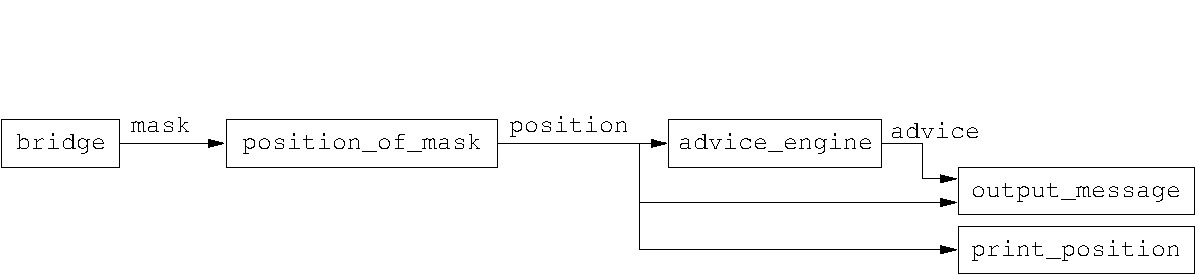
\includegraphics[scale=0.6]{figures/controller}

\pause

\begin{lstrml}
  signal mask default None gather keep_last in
  signal position default None gather keep_last in
  signal advice default None gather keep_last in
  begin
    run Bridge.bridge_async mask ||
    run position_of_mask mask position Ochess.init_position ||
    run advice_engine position advice ||
    run output_messages position advice ||
    run print_position position
  end
\end{lstrml}

\end{frame}

%%%%%%%%%%%%%%%%%%%%%%%%%%%%%%%%%%%%%%%%%%%%%%%%%%%%%%%%%%%%%%%%%%%%%%%%%%%

\begin{frame}[fragile]
\frametitle{Controller: example of process}

\begin{lstrml}
let process output_messages position advice =
  loop
    await position (Some (move, pos)) in
    print_endline ("MOVD "^(Ochess.long_string_of_move move pos));
    match Ochess.game_status pos with
    | Ochess.Win color -> print_endline "ENDG checkmate"
    | Ochess.Draw -> print_endline "ENDG stalemate"
    | Ochess.Play _ -> ()
  end
  ||
  loop
    await advice (Some (pos, smove)) in
    let msg = Ochess.long_string_of_smove pos smove in
    print_endline ("KIBB "^msg)
  end
\end{lstrml}

\end{frame}

%%%%%%%%%%%%%%%%%%%%%%%%%%%%%%%%%%%%%%%%%%%%%%%%%%%%%%%%%%%%%%%%%%%%%%%%%%%

\begin{frame}[fragile]
\frametitle{Why ReactiveML?}

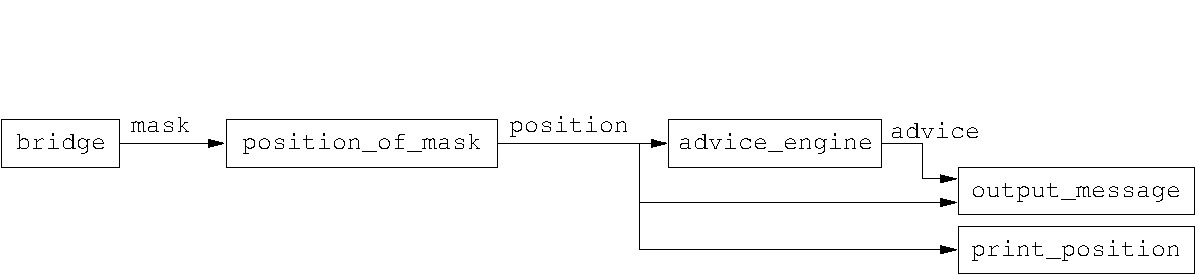
\includegraphics[scale=0.6]{figures/controller}

\begin{lstrml}
  signal mask default None gather keep_last in
  signal position default None gather keep_last in
  signal advice default None gather keep_last in
  begin
    run Bridge.bridge_async mask ||
    run position_of_mask mask position Ochess.init_position ||
    run advice_engine position advice ||
    run output_messages position advice ||
    run print_position position
  end
\end{lstrml}

\end{frame}

%%%%%%%%%%%%%%%%%%%%%%%%%%%%%%%%%%%%%%%%%%%%%%%%%%%%%%%%%%%%%%%%%%%%%%%%%%%

\begin{frame}[fragile]
\frametitle{Controller with reset}

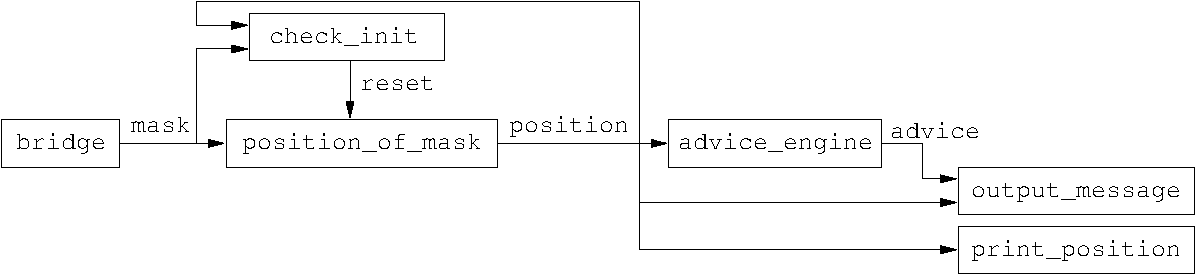
\includegraphics[scale=0.6]{figures/controller-with-reset}

\begin{lstrml}
  signal mask default None gather keep_last in
  signal position default None gather keep_last in
  signal advice default None gather keep_last in
  signal reset default () gather (fun () () -> ()) in
  begin
    run Bridge.bridge_async mask ||
    loop
      do
        run position_of_mask mask position Ochess.init_position
      until reset done
    end ||
    run check_init position mask reset ||
    ...
  end
\end{lstrml}

\end{frame}


%%%%%%%%%%%%%%%%%%%%%%%%%%%%%%%%%%%%%%%%%%%%%%%%%%%%%%%%%%%%%%%%%%%%%%%%%%%
\section{Voice}
%%%%%%%%%%%%%%%%%%%%%%%%%%%%%%%%%%%%%%%%%%%%%%%%%%%%%%%%%%%%%%%%%%%%%%%%%%%

\begin{frame}[fragile]
\frametitle{Voice}

\begin{itemize}
    \item {\scriptsize \verb.MOVD "rnbqkbnr/pppppppp/8/8/8/8/PPPPPPPP/RNBQKBNR w KQkq - 0 0" "e2e4". }
\end{itemize}

\pause

\begin{lstpython}
def pronounce_move(fen_str, uci_str):
    # Move data re-interpreted by python-chess
    board = chess.Board(fen_str)
    move = board.parse_uci(uci_str)

    s = board.san(move) # standard algebraic notation, e.g: "Qxc7"

    s = s.replace("K", "king ")
    s = s.replace("Q", "queen ")
    s = s.replace("R", "rook ")
    s = s.replace("B", "bishop ")
    s = s.replace("N", "knight ")
    s = s.replace("x", " takes ")
    s = s.replace("+", ", check!")
    s = s.replace("#", ", checkmate!")

    say(san)
\end{lstpython}

\end{frame}

%%%%%%%%%%%%%%%%%%%%%%%%%%%%%%%%%%%%%%%%%%%%%%%%%%%%%%%%%%%%%%%%%%%%%%%%%%%
\section{Deliverable}
%%%%%%%%%%%%%%%%%%%%%%%%%%%%%%%%%%%%%%%%%%%%%%%%%%%%%%%%%%%%%%%%%%%%%%%%%%%

\begin{frame}[fragile]
\frametitle{Deliverable}

\begin{center}
  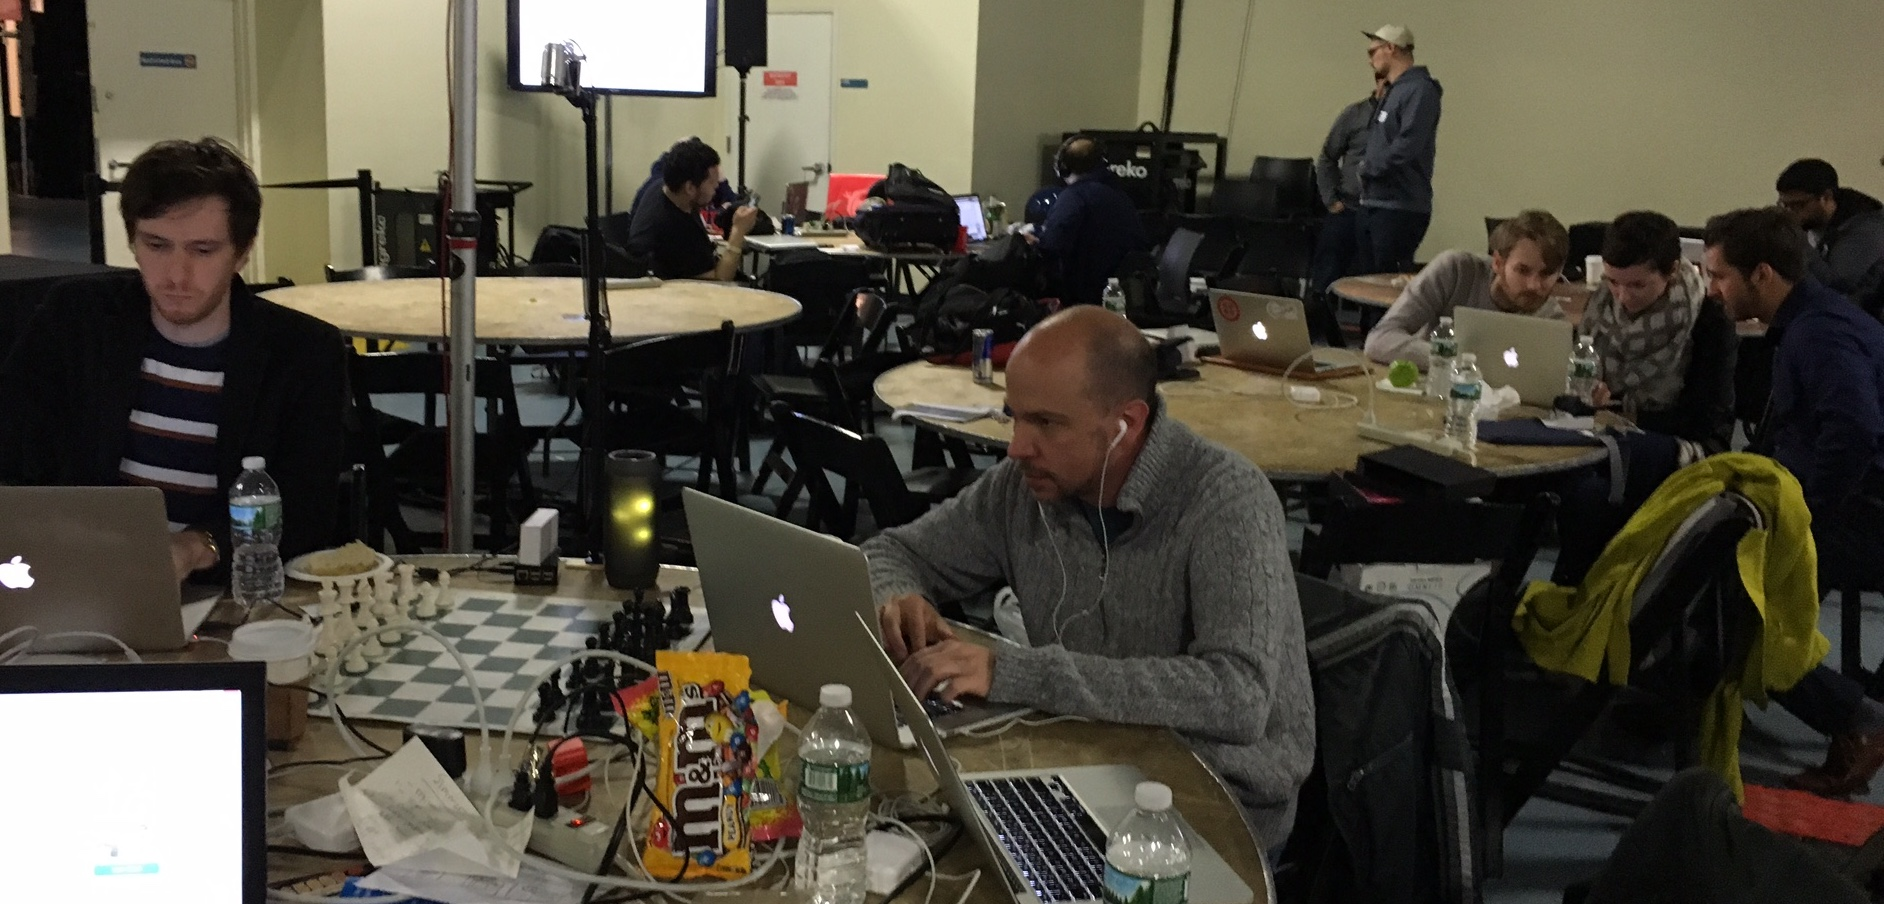
\includegraphics[scale=0.15]{figures/photo-deliverable}
\end{center}

\begin{itemize}
\item Source code: \url{https://github.com/chesseye/chesseye}
  \medskip
\item Web site: \url{http://devpost.com/software/chesseye}
  \medskip
\item Talk: \url{https://youtu.be/bYtGw61YLRk}
  \begin{itemize}
  \item background video: \url{https://vimeo.com/165765674}
  \end{itemize}
\end{itemize}


\end{frame}

%%%%%%%%%%%%%%%%%%%%%%%%%%%%%%%%%%%%%%%%%%%%%%%%%%%%%%%%%%%%%%%%%%%%%%%%%%%

\begin{frame}[fragile]
\frametitle{Great business impact}

\begin{center}
  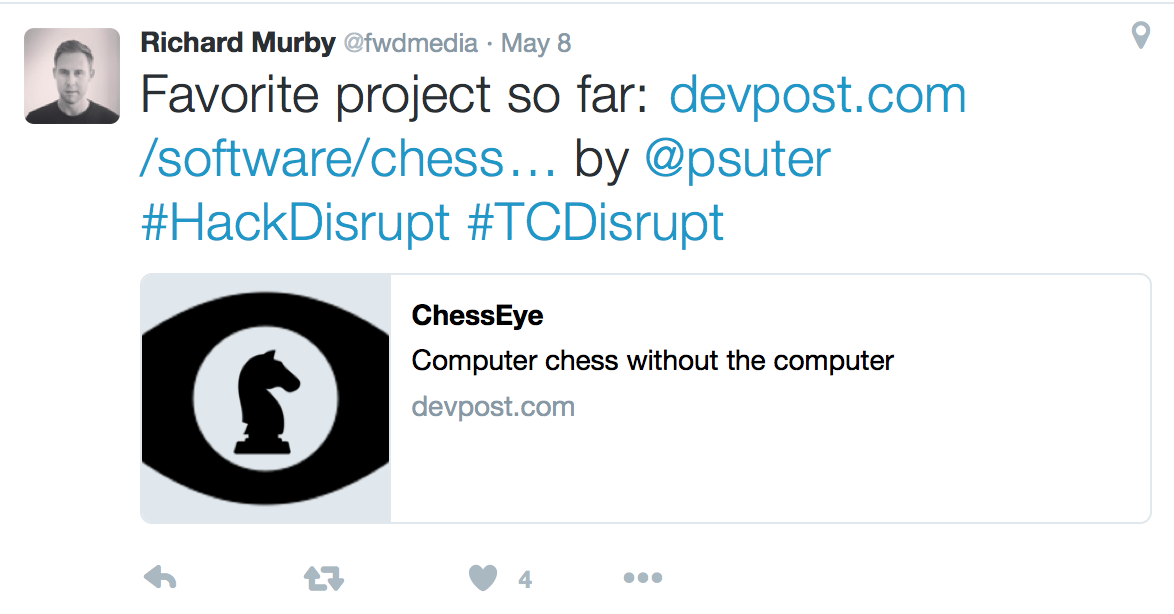
\includegraphics[scale=0.5]{figures/tweet1}\\
  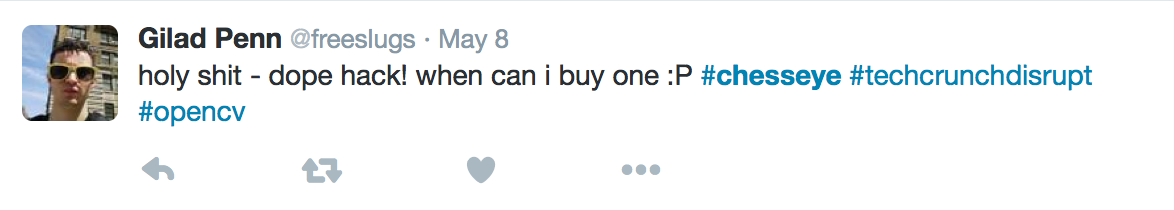
\includegraphics[scale=0.5]{figures/tweet2}
\end{center}

\end{frame}

% %%%%%%%%%%%%%%%%%%%%%%%%%%%%%%%%%%%%%%%%%%%%%%%%%%%%%%%%%%%%%%%%%%%%%%%%%%%

% \begin{frame}[fragile]
% \frametitle{}


% \end{frame}



\end{document}

%%% Local Variables:
%%% mode: pdflatex
%%% TeX-master: "cours"
%%% End:
